\documentclass[14pt,a4paper]{scrartcl}
\usepackage{cmap} % Улучшенный поиск русских слов в полученном pdf-файле
\usepackage[T2A]{fontenc} % Поддержка русских букв
\usepackage[utf8]{inputenc} % Кодировка utf8
\usepackage[english, russian]{babel} % Языки: русский, английский
\usepackage{misccorr}
\usepackage{graphicx}
\usepackage{amsmath}
\usepackage{wrapfig}
\begin{document}
		\begin{tabular}[t]{|l|} 
		\hline
		1. Основные понятия и постулаты термодинамики. Релаксация и\\
		термодинамическое равновесие. Функция состояния – температура, и ее \\
		свойства. Формулировки I-го и II-го начал термодинамики.\\
		\hline
		\end{tabular}\\
	
		\quad  \textit{Температура - } характеристика различной степени нагретости тел.  Это понятие не имеет смысла для одного или малого количества молекул. \textit{Чувственная оценка} температуры сильно зависит от \textit{теплопроводности} тела и применима в очень узком тепловом диапазоне.
		
		\quad Два (или несколько) тела находятся в \textit{термодинамическом равновесии} друг с другом и имеют \textit{одинаковые температуры}, если при контакте между ними не происходят макроскопические изменения.
		
		\quad \textit{Изолированной} или \textit{замкнутой системой} тел называют такую, что не может обмениваться энергией с окружающими телами. Например, система, заключенная в твердую \textit{теплонепроводящую} или \textit{адиабатическую оболочку}.
		
		\quad \textbf{Общее начало термодинамики}. \textit{Каково бы ни было начальное состояние тел изолированной системы, в ней в конце концов установится термодинамическое равновесие, в котором прекратятся все макроскопические процессы.}
		
		\quad Самопроизвольный процесс перехода системы в состояние термодиначеского равновесия называется \textit{релаксацией}, а время, затраченное на такой переход, - \textit{временем релаксации}.
		
		
		
		\quad Если система помещена в адиабатическую оболочку, то единственным способом изменить ее внутреннюю энергию является производство над ней макроскопической работы, что достигается путем изменения внешних параметров.\\
		
		\quad Процесс обмена внутренними энергиями соприкасающихся тел, не сопровождающийся производством макроскопической работы, называется \textit{теплообменом}. Энергия, переданная телу окружающей средой в результате теплообмена, называется \textit{количеством тепла}, или просто \textit{теплом}, полученным телом в таком процессе.
		
		\begin{wrapfigure}[8]{r}{0.2\linewidth} 
			\vspace{-2ex}
			\hspace{5ex}
			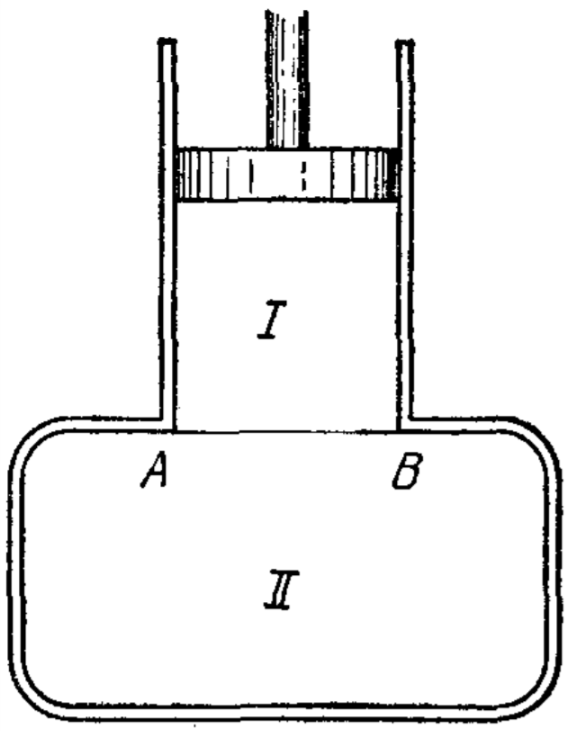
\includegraphics[width=\linewidth]{termostat.png}
		\end{wrapfigure}
		\quad  Пусть термодинамическая система I находится в тепловом контакте с какой-то системой II. Вся система I + II заключена в адиабатическую оболочку, однако, граница AB между системами является теплопроводящей. Система I + II  не может обмениваться теплом с окружающей средой, но теплообмен между I и II может происходить. Допустим, что оболочка системы II жесткая $\Rightarrow$ система II производить работы не может. Система I, напротив, может совершать работу над окружающей средой. Поршень не проводит тепло. 

		\quad Пусть система I + II  перешла из произвольного состояния 1 в другое состояние 2, в результате чего, совершена работа $A_{12}$ над внешними телами. Эту работу совершала только система I. Т.к. составная система I + II адиабатически изолирована, то $$A_{12} = (U_1 + U_1')-(U_2+U_2'),$$ где $U - $ внутренняя энергия системы I, а $U'-$ системы II. Т.к. нас интересует поведение только системы I, перепишем это соотношение так: $$A_{12} = U_1 - U_2 + (U_1' - U_2').$$
		
		\quad Уменьшение внутренней энергии системы II есть, по определению, количество тепла \textit{Q}, полученное системой I в рассматриваемом процессе. Тогда по определению $$Q = U_1' - U_2' = -\partial U',$$ и предыдущее соотношение примет вид \begin{equation}\label{*} Q = U_2 -U_1 + A_{12}. \end{equation}
		Это уравнение дает математическую формулировку \textbf{первого начала термодинамики}. Оно утверждает, что\textit{ тепло Q, полученное системой, идет на приращение ее внутренней энергии $\partial U = U_2 -U_1$ и на производство внешней работы.}
		
		\quad В случае, если оболочка II не является жесткой, то система II может совершать работу. Если $A_{\text{полн}}-$ полная работа системы I + II, то $$A_{\text{полн}} = U_1 - U_2 + (U_1' -U_2').$$
		
		\quad Полная работа слагается из работы $A_{12}$ системы I и работы $A_{12}'$ системы II: $A_{\text{полн}} = A_{12} +A_{12}'$. Поэтому предыдущее соотношение по-прежнему можно записать в виде (*), если \textit{Q} определить выражением $$Q = U_1' - U_2' - A_{12}'.$$
		
		\quad Для бесконечно малого или элементарного квазистатического процесса уравнение (*) принимает вид $$\delta Q = dU +\delta A$$ или $$\delta Q = dU + PdV.$$ 
		
		\quad Если процесс круговой, то $U_2 = U_1 \Rightarrow Q = A$. Т.е. в круговом процессе все тепло, полученное системой, идет на производство внешней работы.
		
		\quad Если $U_1 + U_2$ и $Q = 0$, то $A = 0$. Это значит, что невозможен процесс, единственным результатом которого является производство работы без каких бы то ни было изменений в других телах $\Rightarrow$ вечный двигатель не существует.\\
		
		\begin{wrapfigure}[8]{r}{0.4\linewidth} 
			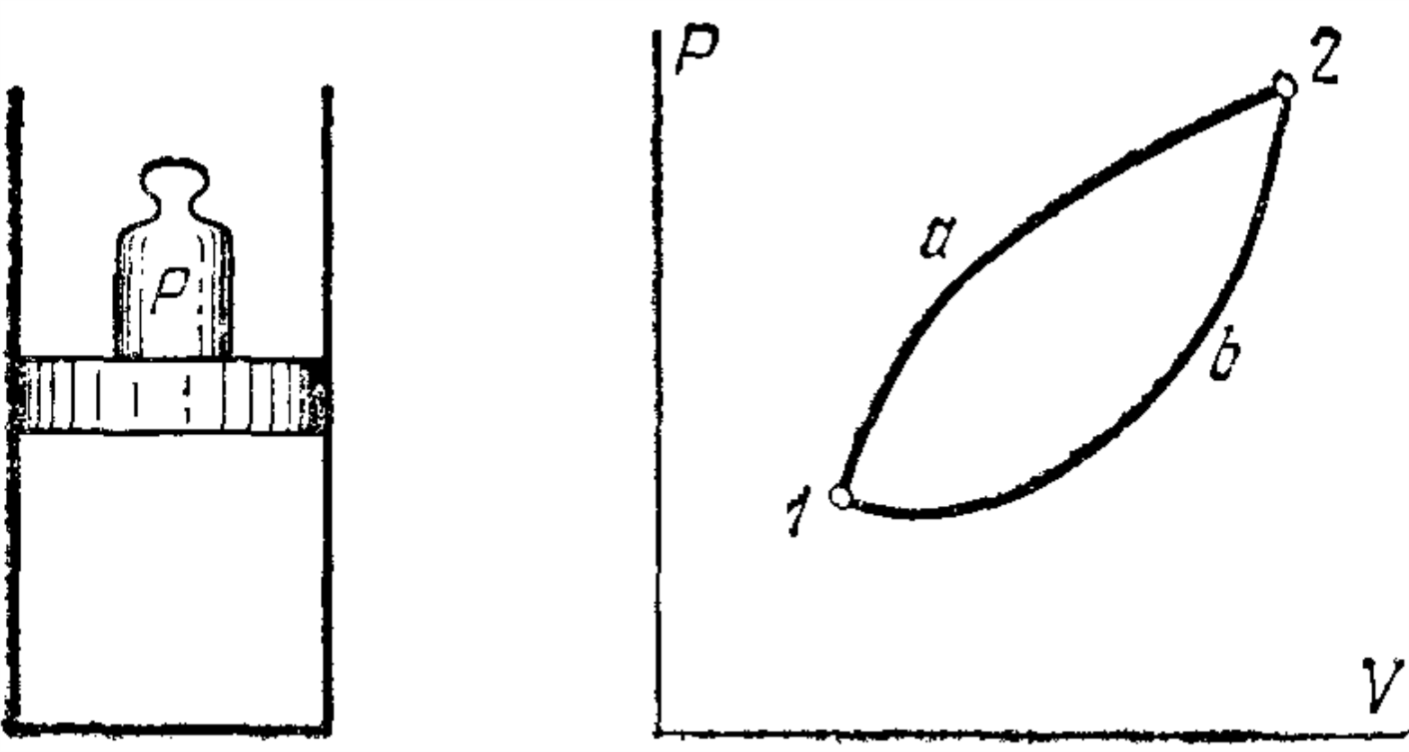
\includegraphics[width=\linewidth]{warm_machine.png}
		\end{wrapfigure}
		\quad Рассмотрим работу тепловой машины. В цилиндре машины помещается газ, называемый \textit{рабочим телом}. Пусть на VP диаграмме  1 - начальное состояние рабочего тела. Приведем дно цилиндра в тепловой контакт с нагревателем, т.е. телом, температура которого выше температуры газа в цилиндре. Газ будет нагреваться и расширяться - кривая 1а2. Рабочее вещество получит от нагревателя тепло $Q_1$ и совершит положительную работу $A_1$. По первому началу $$Q_1  = U_2-U_1+A_1.$$
		
		\quad Теперь надо вернуть поршень в исходное положение, т.е. сжать газ так, чтобы работа $A_2$, затраченная на сжатие, была меньше $A_1$. С этой целью приведем дно цилиндра в тепловой контакт с холодильником, т.е. телом, температура которого ниже температуры газа в цилиндре, и сожмем газ по пути 2b1. В результате газ вернутся в исходное состояние I. При этом он отдаст холодильнику тепло $Q_2$. По первому началу $$-Q_2 = U_1 - U_2 - A_2.$$ Сложив с $Q_1$ получим $$Q_1 - Q_2 = A_1 - A_2.$$
		
		\quad Т.о. тепловая машина совершила круговой процесс, в результате которого нагреватель отдал тепло $Q_1$, холодильник получил тепло $Q_2$, тепло $Q = Q_1 - Q_2$ пошло на производство работы $A_1 - A_2$. Отношение $$\eta = \dfrac{A}{Q_1} = \dfrac{Q_1-Q_2}{Q_1}$$ называется \textit{коэффициентом полезного действия} тепловой машины.
		
		\quad\textit{Постулат второго начала термодинамики} гласит о том, что невозможно построить перпетум мобиле второго рода (идеальная тепловая машина, которая превращает в работу всю теплоту, заимствованную от одного теплового резервуара. Работает за счет практически неисчерпаемых запасах внутренней энергии океанов, атмосферы и т.д.). 
		
		\quad Постулат Томсона: \textit{Невозможен круговой процесс, единственным результатом которого было бы производство работы за счет /охлаждения теплового резервуара/ уменьшения внутренней энергии теплового резервуара.} Тепловой резервуар - тело или система тел, находящаяся в состоянии термодинамического равновесия и обладающая запасом внутренней энергии.
		
		\quad Постулат Клаузиуса: \textit{теплота(внутренняя энергия тела) не может самопроизвольно переходить от тела менее нагретого к телу более нагретому.} (Невозможно сделать это так, чтобы в природе не произошло никаких изменений)\\
		
		\begin{tabular}[t]{|l|ll|} 
			\hline
			 2. Формулировка II-го начала термодинамики по Клаузиусу. Цикл и \\теорема
			 Карно.\\
			 \hline
		 \end{tabular}\\
		
		\quad Постулат Клаузиуса: \textit{теплота(внутренняя энергия тела) не может самопроизвольно переходить от тела менее нагретого к телу более нагретому.} (Невозможно сделать это так, чтобы в природе не произошло никаких изменений)\\
		
		\quad Если в результате какого-либо процесса система переходит из состояния А в другое состояние В и если возможно вернуть ее хотя бы одним способом в исходное состояние А и притом так, чтобы во всех остальных телах не произошло никаких изменения, то этот процесс называется \textit{обратимым}. Если же это сделать невозможно, то	процесс называется \textit{необратимым}. Из постулата Клаузиуса следует необратимость процесса передачи теплоты от более нагретого к менее нагретому при тепловом контакте.\\
		
		\begin{wrapfigure}[8]{r}{0.3\linewidth} 
				\vspace{-2ex}
			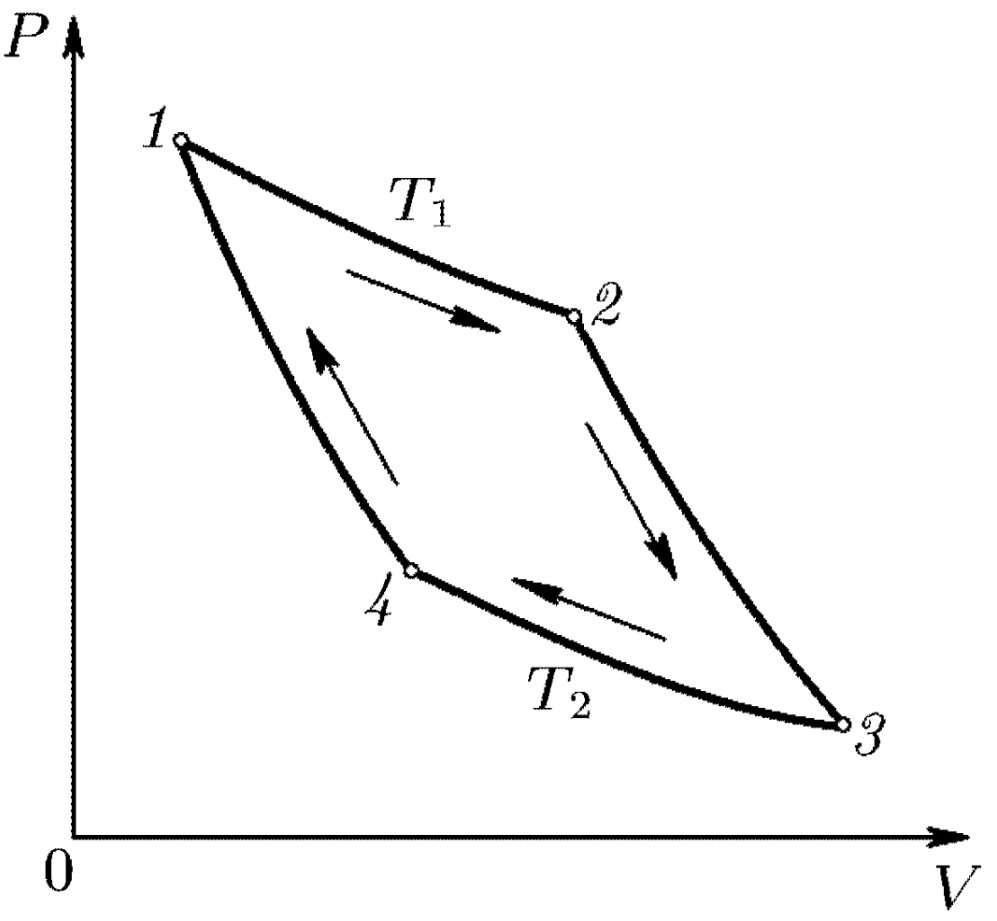
\includegraphics[width=\linewidth]{karno.png}
		\end{wrapfigure}
		\quad \textit{Круговой процесс}, или \textit{процесс Карно} - это квазистатический процесс, в котором систему можно приводить в тепловой контакт	с двумя тепловыми резервуарами, имеющими постоянные температуры $T_1$ и $T_2$. В дальнейшем предполагается, что $T_1 > T_2$. Тепловой резервуар с более высокой температурой $T_1$ называется \textit{нагревателем} , а с более низкой температурой $T_2 -$	\textit{холодильником}. Цикл Карно заключается в следующем. Сначала система, имея температуру $T_1$ приводится в тепловой контакт с нагревателем. Затем, бесконечно медленно уменьшая внешнее давление, ее заставляют квазистатически расширяться по изотерме 12.	При этом она заимствует теплоту $Q_1$ от нагревателя и производит работу $A_{12}$ против внешнего давления. После этого систему адиабатически изолируют и заставляют квазистатически расширяться по адиабате 23, пока ее температура не достигнет температуры холодильника $T_2$. При адиабатическом расширении система также совершает некоторую работу $A_{23}$ против внешнего давления. В состоянии 3 систему приводят в тепловой контакт с холодильником и непрерывным увеличением давления изотермически сжимают ее до некоторого состояния 4.	При этом над системой производится работа (т. е. сама система совершает отрицательную работу $A_{34}$), и она отдает холодильнику некоторое количество теплоты $Q_2$. Состояние 4 выбирается так, чтобы можно было квазистатическим сжатием по адиабате 14 вернуть систему в исходное состояние 1. Для этого надо, разумеется, над системой совершить работу (т. е. сама
		система должна произвести отрицательную работу $A_{41}$). В результате кругового процесса Карно внутренняя энергия системы не изменится, а поэтому произведенная ею работа $A = A_{12} + A_{23} + A_{34} + A_{41} = Q_1 - Q_2$. Коэффициент полезного действия $\eta$ цикла Карно определяется соотношением $$\eta = \dfrac{A}{Q_1} = \dfrac{Q_1-Q_2}{Q_1},$$ из которого следует $$Q_2 = (1-\eta)Q_1.$$\\
		
		\quad \textbf{Теорема Карно}: \textit{коэффициент полезного действия тепловой машины, работающей по циклу Карно, зависит только от температур $T_1$ и $T_2$ нагревателя и холодильника, но не зависит от устройства машины, а также от вида используемого рабочего вещества.}
		
		\quad Доказательство. Рассмотрим две машины Карно, имеющие общий нагреватель при температуре $T_1$и общий холодильник при температуре $T_2$. Пусть КПД первой машины равен $\eta$, а второй $\eta'$. Допустим, что $\eta > \eta'$, и покажем, что это допущение приводит к противоречию с постулатом второго начала термодинамики. Цикл Карно —  квазистатический, а потому он может совершаться как в прямом, так и в обратном направлении, т. е. производить работу. Пусть в результате $m$ циклов она отберет от нагревателя теплоту $Q_1$, передаст холодильнику теплоту $Q_2$ и произведет работу $А =	Q_1 -Q_2$, например, поднимет груз. Остановим после этого первую машину и используем потенциальную энергию поднятого груза, чтобы привести в действие вторую машину в обратном направлении. Вторая машина Карно будет, следовательно, работать как холодильная машина. Пусть в результате $m'$ циклов она заберет теплоту $Q_2'$ от холодильника и передаст теплоту $Q_1'$ нагревателю; при этом над машиной будет совершена работа $А' =	Q_1' -Q_2'$. Результат действия $m$ циклов первой и $m'$ циклов второй машины представится схемой.\\
		\text{\qquad нагреватель отдал теплоту $Q_1 - Q_1'$,}\\
		\text{\qquad холодильник отдал теплоту $Q_2' - Q_2$,}\\
		\text{\qquad машина совершила работу} $$A-A' = (Q_1 -Q_2) - (Q_1'-Q_2') = \eta Q_1 - \eta' Q_1'.$$
		\quad Для постулата Томсона-Планка выберем целые числа $m$ и $m'$ так, чтобы $Q_1 - Q_1'=0$. Действительно, $Q_1 = mq_1, Q_1 = m'q_1'$, где $q_1 - $ количество теплоты, полученное первой машиной от нагревателя в результате одного цикла, а $q_1' - $ количество теплоты, отданное тому же нагревателю второй машиной также в результате одного цикла. Если $q_1$ и $q_1'$ соизмеримы, то всегда можно подобрать целые числа $m$ и $ m' $ так, чтобы $ mq_1 - m'q_1' = 0 $, т.е. $ Q_1 - Q_1' = 0 $. Если же эти величины не соизмеримы, то целые числа $m$ и $ m' $ можно выбрать настолько большими, чтобы это равенство выполнялось с какой угодно заранее заданной точностью. Поэтому физически всегда возможно выбрать целые числа $m$ и $ m' $ так, чтобы $ Q_1 - Q_2' =0 $. Тогда результат кругового процесса предсавится в виде\\
		\text{\qquad состояние не изменилось,}\\
		\text{\qquad холодильник отдал теплоту $ Q_2' - Q_2 = (\eta - \eta')Q_1 > 0 $,}\\
		\text{\qquad машина совершила работу $\eta Q_1 - \eta' Q_1' = (\eta - \eta')Q_1 > 0$.}\\
		
		\quad Т.о., единственным результатом кругового процесса будет производство работы $ (\eta - \eta')Q_1 > 0 $ за счет эквивалентного количество теплоты, заимствованного от холодильника. Это процесс Томсона-Планка, возможность которого противоречит постулату второго начала термодинамики. Поэтому предположение $\eta > \eta'$ неверно - так же неверно предположение $\eta' > \eta $. Чтобы убедиться в этом, нужно заставить вторую машину пройти цикл Карно в прямом, а первоую - в обратном направлении и повторить рассуждение $\Rightarrow\quad \eta = \eta'$. Теорема Карно доказана.
		
		
		\begin{tabular}[t]{|l|ll|} 
			\hline
			3. Формулировка II-го начала термодинамики по Клаузиусу. Цикл Карно и\\
			абсолютная термодинамическая шкала температур.\\
			\hline
		\end{tabular}\\
		
		\quad Постулат Клаузиуса: \textit{теплота(внутренняя энергия тела) не может самопроизвольно переходить от тела менее нагретого к телу более нагретому.} (Невозможно сделать это так, чтобы в природе не произошло никаких изменений)\\
 		
 		\begin{wrapfigure}[8]{r}{0.3\linewidth} 
 			\vspace{-2ex}
 			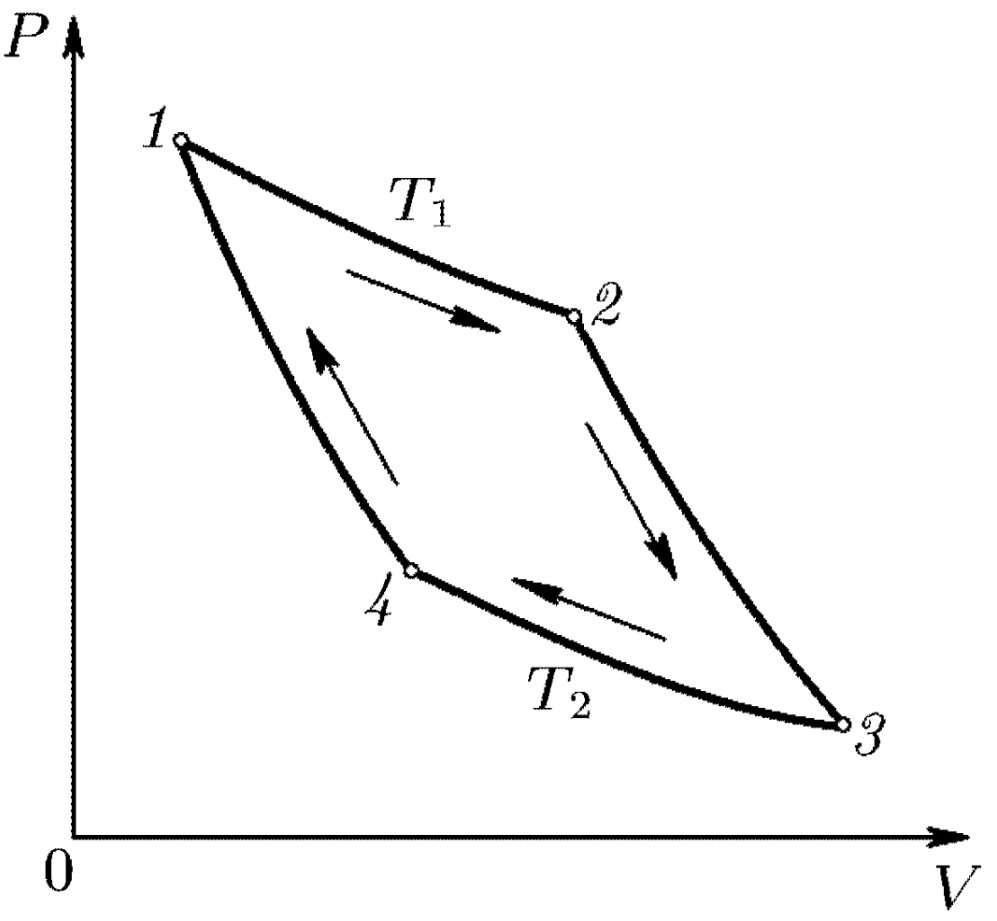
\includegraphics[width=\linewidth]{karno.png}
 		\end{wrapfigure}
 		\quad \textit{Круговой процесс}, или \textit{процесс Карно} - это квазистатический процесс, в котором систему можно приводить в тепловой контакт	с двумя тепловыми резервуарами, имеющими постоянные температуры $T_1$ и $T_2$. В дальнейшем предполагается, что $T_1 > T_2$. Тепловой резервуар с более высокой температурой $T_1$ называется \textit{нагревателем} , а с более низкой температурой $T_2 -$	\textit{холодильником}. Цикл Карно заключается в следующем. Сначала система, имея температуру $T_1$ приводится в тепловой контакт с нагревателем. Затем, бесконечно медленно уменьшая внешнее давление, ее заставляют квазистатически расширяться по изотерме 12.	При этом она заимствует теплоту $Q_1$ от нагревателя и производит работу $A_{12}$ против внешнего давления. После этого систему адиабатически изолируют и заставляют квазистатически расширяться по адиабате 23, пока ее температура не достигнет температуры холодильника $T_2$. При адиабатическом расширении система также совершает некоторую работу $A_{23}$ против внешнего давления. В состоянии 3 систему приводят в тепловой контакт с холодильником и непрерывным увеличением давления изотермически сжимают ее до некоторого состояния 4.	При этом над системой производится работа (т. е. сама система совершает отрицательную работу $A_{34}$), и она отдает холодильнику некоторое количество теплоты $Q_2$. Состояние 4 выбирается так, чтобы можно было квазистатическим сжатием по адиабате 14 вернуть систему в исходное состояние 1. Для этого надо, разумеется, над системой совершить работу (т. е. сама
 		система должна произвести отрицательную работу $A_{41}$). В результате кругового процесса Карно внутренняя энергия системы не изменится, а поэтому произведенная ею работа $A = A_{12} + A_{23} + A_{34} + A_{41} = Q_1 - Q_2$. Коэффициент полезного действия $\eta$ цикла Карно определяется соотношением $$\eta = \dfrac{A}{Q_1} = \dfrac{Q_1-Q_2}{Q_1},$$ из которого следует $$Q_2 = (1-\eta)Q_1.$$\\
		
		\begin{wrapfigure}[8]{r}{0.3\linewidth} 
			\vspace{-5ex}
			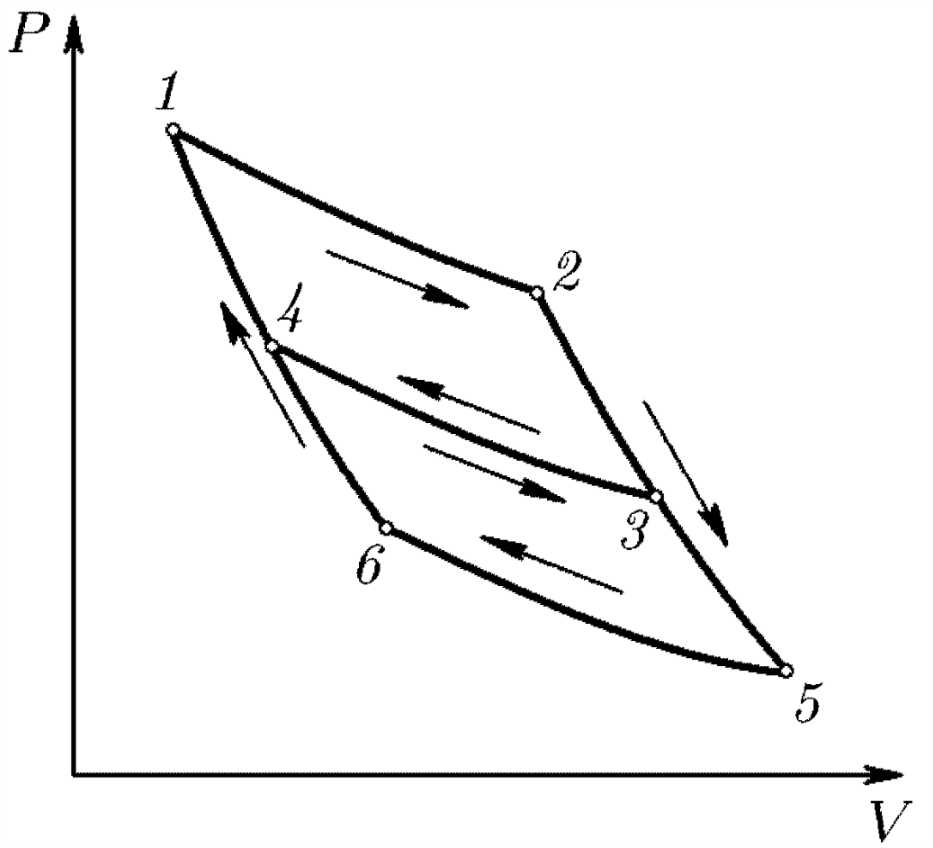
\includegraphics[width=\linewidth]{shkala.png}
		\end{wrapfigure}
		\quad Чтобы построить \textit{термодинамическую шкалу температур}, введем универсальную функцию температур $t_1$ и $t_2$: $$\dfrac{Q_1}{Q_2} = \phi(t_1, t_2).$$
		\quad Определим общий вид функции $ \phi(t_1, t_2) $. Для этого возьмем три тепловых резервуара, температуры которых поддерживаются постоянными. Эмпирические температуры этих резервуаров обозначим $t_1, t_2, t_3$. Используя их в качестве нагревателей и холодильников проведем три цикла Карно. Предполагается, что $t_1, t_2, t_3 - $ температуры на изотермах 12, 43, 65. Для циклов Карно 1234 и 4356 можно написать $$\dfrac{Q_1}{Q_2} = \phi(t_1, t_2), \quad \dfrac{Q_2}{Q_3} = \phi(t_2, t_3).$$ Исключив отсюда теплоту $Q_2$, получим $$\dfrac{Q_1}{Q_3} =\phi(t_1, t_2) \phi(t_2, t_3).$$  Но эти два цикла, эквивалентны циклу Карно 1256. Это происходит потому, что по изотерме 43 проходим дважды в противоположных направлениях и она может быть исключена из рассмотрения. Тогда $$\dfrac{Q_1}{Q_3} = \phi(t_1, t_3).$$ Сравнивая это соотношение с предыдущим, получим $$\phi(t_1, t_2)\phi(t_2, t_3) = \phi(t_1, t_3),$$ откуда $$\phi(t_1, t_2) = \dfrac{\phi(t_1, t_3)}{\phi(t_2, t_3)},$$ или  $$\dfrac{Q_1}{Q_2} = \dfrac{\phi(t_1, t_3)}{\phi(t_3, t_3)}.$$ 
		
		\quad Такое соотношение справедливо при любом значении аргумента $t_3$. Можно фиксировать  $t_3$, не меняя значения самого отношения $\Rightarrow$ числитель в правой части последней формулы будет функцией одного аргумента $t_1$. Обозначим эту функцию через $\Theta(t_1)$. Знаменатель по аналогии. $$\dfrac{Q_1}{Q_2} = \dfrac{\Theta(t_1)}{\Theta(t_2)}.$$
		
		\quad Т.о. $ \phi(t_1, t_2) $ есть отношение значений одной и той же функции $\Theta(t)$ при $t = t_1$ и $t = t_2$.  Величину $\Theta(t)$ называют \textit{абсолютной термодинамическрй температурой}. Отношение двух термодинамических температур $\Theta_1 \equiv \Theta(t)$ и $\Theta_2 \equiv \Theta(t_2)$ определяется соотношением \begin{align}\dfrac{\Theta_1}{\Theta_2} = \dfrac{Q_1}{Q_2}.\tag{*}\end{align}
		
		\quad Т.к. соотношение (*) не зависит от $t_3$, то температуры $\Theta_1$ и $\Theta_2$ не определяются однозначно, т.к. $\Theta(t) = \phi(t, t_3)$, где $t_3$ произвольный $\Rightarrow$ термодинамические температуры будут иметь разные значения при различном выборе этого параметра. Вместо $\Theta(t)$ введем $\Theta'(t) = \psi(t_3)\Theta(t)$, где $\psi(t_3)$ - произвольная функция. От этого значение (*) не изменится. Но придавая параметру $t_3$ различные значения получим бесконечное множество температурных шкал, отличающихся друг от друг масштабами единицы температуры.
		
		\quad Для определения $\Theta$ возьмем две постоянные температурные точки, например нормальную точку плавления льда $\Theta_{\text{п}}$ и нормальную точку кипения воды  $\Theta_{\text{к}}$, а соответсвующие им количества теплоты в цикле Карно - $Q_{\text{п}}$ и $Q_{\text{п}}$. Фиксируем значение разности $\Theta_{\text{к}} - \Theta_{\text{п}}$, например примем, что она равна 100  градусам $\Rightarrow$ имеем 100 равных частей между точками, каждая из которых называлась раньше градусом Кельвина, а теперь - просто кельвином. Из уравнений $$\dfrac{\Theta_{\text{к}}}{\Theta_{\text{п}}} = \dfrac{Q_{\text{к}}}{Q_{\text{п}}}, \quad \Theta_{\text{к}} - \Theta_{\text{п}} = 100$$ можно в отдельности вычислить  $ \Theta_{\text{к}}  $ и $ \Theta_{\text{п}} $(373,15 К и 273,15 К). Для этого надо измерить отношение $\dfrac{Q_{\text{к}}}{Q_{\text{п}}}$. 
		
		\quad Термодинамическую температуру $\Theta$ любого тела можно вычислить по формуле $$\dfrac{\Theta}{\Theta_{\text{п}}}=\dfrac{Q}{Q_{\text{п}}},$$ если предварительно провести цикл Карно между данным телом и тающим льдом и измерить соответствующие количества теплоты $Q$ и $Q_{\text{п}}$. Построенная таким образом температурная шкала называется \textit{абсолютной термодинамической шкалой температур}.\\
		
		
		\begin{tabular}[t]{|l|ll|} 
			\hline
			4. Формулировка II-го начала термодинамики по Клаузиусу. Неравенство \\Клаузиуса.
\\
			\hline
		\end{tabular}\\
	
	\quad Постулат Клаузиуса: \textit{теплота(внутренняя энергия тела) не может самопроизвольно переходить от тела менее нагретого к телу более нагретому.} (Невозможно сделать это так, чтобы в природе не произошло никаких изменений)\\
	
	\begin{wrapfigure}[8]{r}{0.3\linewidth} 
		\vspace{-5ex}
		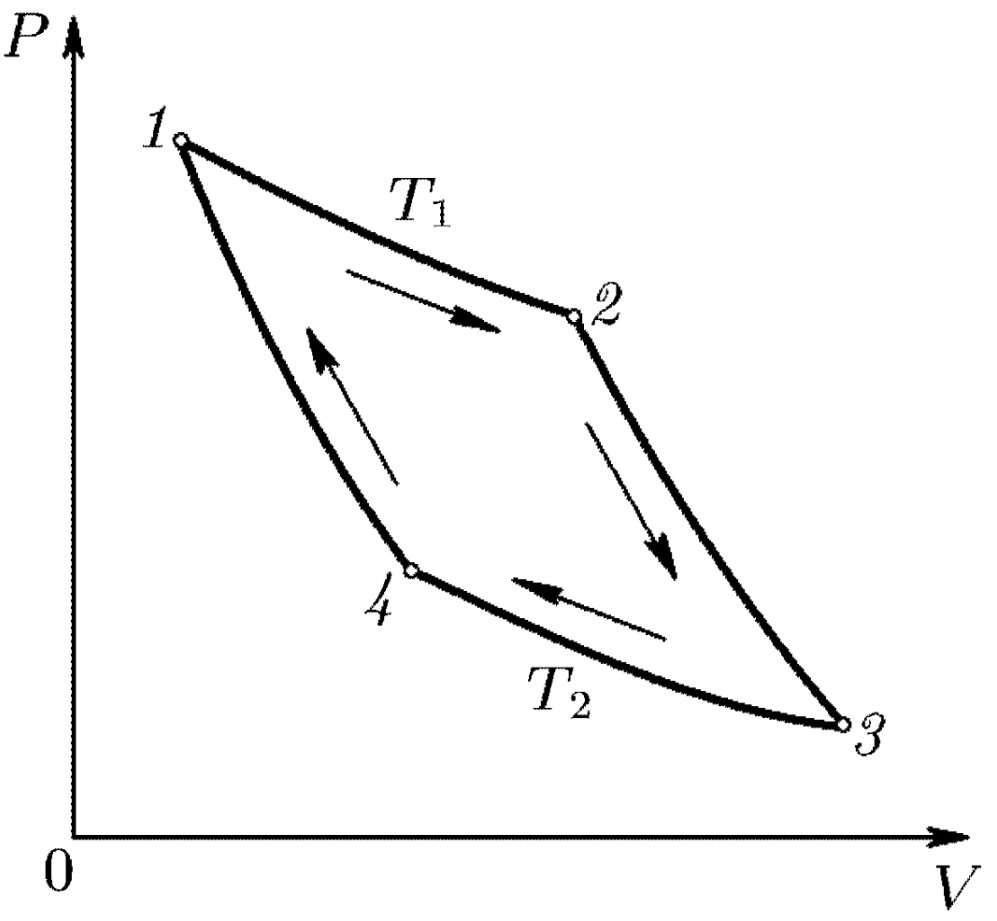
\includegraphics[width=\linewidth]{karno.png}
	\end{wrapfigure}
	\quad Рассмотрим произвольную термодинамическую систему I, которая может обмениваться теплом с двумя тепловыми резервуарами $R_1$ и $R_2$. Их температуры $T_1$ и $T_2$. Т.о., мы не различаем кто нагреватель, а кто холодильник. Количество теплоты, отданное тепловым резервуаром (т.е. полученное системой II) положительно.
	
	\quad Заставим работать обратимую машину Карно между резервуарами $R_1$ и $R_2$, но чтобы ее наличие не влияло на круговой процесс в системе I, присоединяем ее \textit{после} завершения процесса. Тогда резервуры $R_1$ и $R_2$ начнут обмениваться теплом только с машиной Карно. Пусть сама машина Карно совершила круговой процесс, в ходе которого она заимствовала теплоту $Q_1'$ от резервуара $R_1$ и $Q_2'$ от $R_2$. Т.к. машина Карно обратима, то она может работать как двигатель или холодильник, а изотерма 12 в цикле Карно может быть взята сколь угодно короткой и можно получить сколь угодно большую работу $\Rightarrow$ машина Карно позволяет получать как положительную, так и отрицательную работу \textit{наперед заданной величины} $\Rightarrow$ $Q_1'$ или $Q_2'$ может быть произвольным (больше или меньше нуля). 
	
	\quad Объединим машину карно и систему I (соответственно и их круговые процессы в один круговой). Тогда в этом процессе сложная система\\
	\text{\qquad получила от $R_1$ теплоту $Q_1 + Q_1'$}\\
	\text{\qquad получила от $R_2$ теплоту $Q_2 + Q_2'$}\\
	\text{\qquad совершила работу $A = Q_1 + Q_1' +Q_2 +Q_2'$.}\\
	
	Выберем $Q_1' $ так, чтобы $A = Q_1 + Q_1' +Q_2 +Q_2' = 0$, или $Q_1 +Q_1' = -(Q_2+Q_2')$. Тогда единственным результатом кругового процесса будет передача теплоты $Q_1 +Q_1'$  от $R_1$ к $R_2$. Теплоту $Q_1'$ можно найти из условия $A = 0$, если воспользоваться соотношением $$\dfrac{Q_1'}{T_1}=\dfrac{Q_2'}{T_2}=0.$$ Это дает $$Q_1 +Q_1' +Q_2 - \dfrac{T_2}{T_1}Q_1' = 0.$$ Определив отсюда $Q_1'$ находим $$Q_1 +Q_1' = \dfrac{T_1T_2}{T_2 - T_1}(\dfrac{Q_1}{T_1}+\dfrac{Q_2}{T_2}).$$ Если $T_1 > T_2$, то согласно постулату Клаузиуса должно быть $Q_1 +Q_1' \geqslant 0$. Если же $T_1 < T_2$, то должно быть $Q_1 +Q_1' \leqslant 0$. Т.к. абсолютные температуры существенно положительны, то приходим к \textit{неравенству Клаузиуса} $$\boxed{\dfrac{Q_1}{T_1}+\dfrac{Q_2}{T_2}\leqslant 0.}$$\\
	
	
	\begin{tabular}[t]{|l|ll|} 
		\hline
		5. Равенство Клаузиуса для квазистатического процесса. Энтропия - функция\\
		состояния, и $\delta Q = T dS$. Закон возрастания энтропии для адиабатически\\
		изолированной системы.\\
		\hline
	\end{tabular}\\
	
	\quad Допустим, что круговой процесс, совершаемый системой - \textit{квазистатический}. Неравенство Клаузиуса $$\oint \dfrac{\delta Q}{T}\leqslant 0$$ справедливо и для такого процесса. Только под $T$ теперь температура \textit{самой системы}, т.к. обе температуры одиниковы.
	
	\quad Квазистатический процесс обратим. Для обратного процесса также справедливо неравенство Клаузиуса $\oint \dfrac{\delta' Q}{T}\leqslant 0$, где $\delta' Q$ - элементарные количества теплоты, получаемые системой на отдельных участках такого обратного процесса. Т.к. система проходит через те же равновесные состояния, что и в прямом процессе, то $\delta' Q = -\delta Q$, а потому $\oint \dfrac{\delta Q}{T}\geqslant 0$. Т.о., \textit{для квазистатического процесса неравенство Клаузиуса переходит в равенство} $$\oint\limits_{\text{квст}} \dfrac{\delta Q}{T} = 0$$
	
	\quad Пусть система может переходить их начального состояния 1 в конечное 2 несколькими способами, каждый их которых - квазистатический процесс. Возьмем пути I и II. Объединим их в один квазистатический круговой процесс 1I2II1. Применим к нему равенство Клаузиуса: $$\int\limits_{1 I 2} \dfrac{\delta Q}{T} +\int\limits_{2 II 1} \dfrac{\delta Q}{T} = 0,$$ или  $$\int\limits_{1 I 2} \dfrac{\delta Q}{T} - \int\limits_{1 II 2} \dfrac{\delta Q}{T} = 0,$$ или наконец, $$\int\limits_{1 I 2} \dfrac{\delta Q}{T} = \int\limits_{1 II 2} \dfrac{\delta Q}{T} .$$
	\begin{wrapfigure}[6]{r}{0.3\linewidth} 
		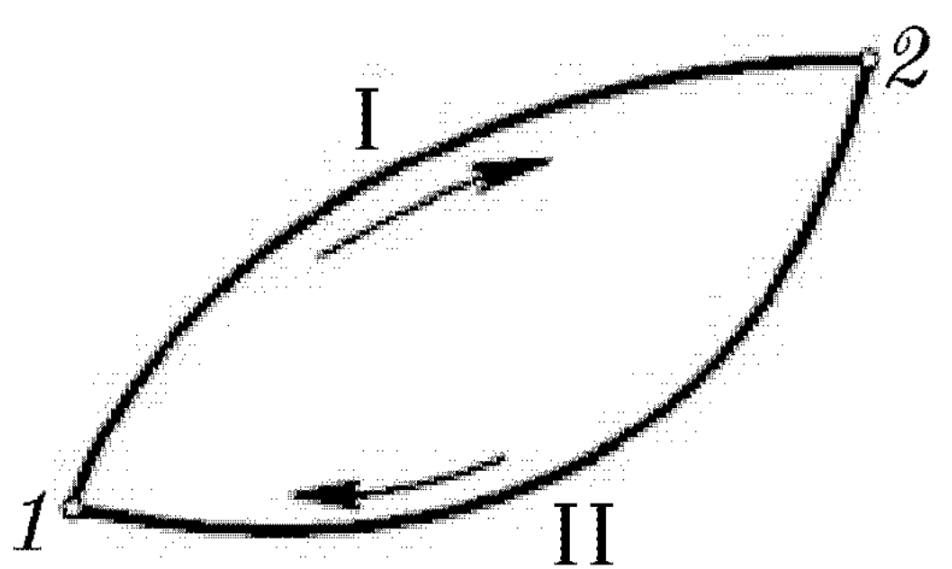
\includegraphics[width=\linewidth]{entropy.png}
	\end{wrapfigure}

	\quad Количество теплоты, полученное системой, деленное на абсолютную температуру $Т$, при которой оно было получено, иногда называют \textit{приведенным количеством теплоты}. Величина $\dfrac{\delta Q}{T}$ - элементарное приведенное количество теплоты, полученные в бесконечно малом процессе, а $\int \dfrac{\delta Q}{T}$ - приведенное количество теплоты в конечном процессе. Равенство клаузиуса: \textit{приведенное количество теплоты, не зависит от пути перехода, а определяется лишь начальным и конечным состояниями системы.}
	
	\quad \textit{\textbf{Энтропия} системы - функция ее состояния, определенная с точностью до произвольной постоянной. Разность энтропий в двух равновесных состояниях 2 и 1, по определению, равна приведенному количеству теплоты, которое надо сообщить системе, чтобы перевести ее из состояния 1 в состояние 2 по любому квазистатическому пути.} Т.о., $S_1$ и $S_2$ - энтропии в состояниях 1 и 2, тогда по определению $$S_2 - S_1 = \int\limits_{1\to2} \dfrac{\delta Q}{T}.$$ Значение произвольной постоянной, с которой определена энтропия, не играет роли. Для дифференциала функции $S$ имеем $$dS = (\dfrac{\delta Q}{T})_{\text{квст}}$$ Тогда если $\delta Q$ - элементарное количество теплоты, квазистатически полученное системой, то после деления на $T$ оно переходит в полный дифференциал функции состояния - энтропии.\\
	
	\quad Допустим, система переходит из равновесного состояния 1 в равновесное состояние 2, но процесс перехода необратим. Вернем систему из состояния 2 в исходное 1 квазистатически по какому-либо пути II. На основании неравенства Клаузиуса запишем $$\oint \dfrac{\delta Q}{T} \equiv \int\limits_I \dfrac{\delta Q}{T} + \int\limits_{II} \dfrac{\delta Q}{T} \leqslant 0.$$ Т.к. процесс II квазистатический, то $$\int\limits_{II}\dfrac{\delta Q}{T}=S_1-S_2.$$ Поэтому неравенство Клаузиуса принимает вид \begin{align} S_2 - S_1 \geqslant \int\limits_{1\to2}\dfrac{\delta Q}{T}.\tag{*}\end{align} Здесь $T$ - температура окружающей среды, при которой она отдает системе количество теплоты $\delta Q$.
	
	\quad Если система адиабатически изолирована, то $\delta Q = 0$, и интеграл (*) обращается в нуль. Тогда $$S_2 \geqslant S_1.$$  \textbf{Закон возрастания энтропии.} Т.о., \textit{энтропия адиабатически изолированной системы не может убывать; она либо возрастает, либо остается постоянной.}\\
	
		\begin{tabular}[t]{|l|ll|} 
		\hline
		6. Соотношение $dU = TdS - PdV$ как следстие I-го и II-го начал термоди-\\намики	для квазистатических процессов. Эквивалентность $PV -$ и $TS-$ \\плоскостей. Соотношения между производными термодинамических величин. 	\\Например, доказать что	$(\frac{\partial U}{\partial V})_T = T(\frac{\partial P}{\partial T})_V - P.$	\\
		\hline
	\end{tabular}\\\\

	\quad Термодинамические соотношения получаются, в общем, двумя способами.
	\begin{enumerate} \item С помощью \textit{якобианов}: 
	$$\dfrac{\partial (A, B)}{\partial (x,y)} = \biggl(\dfrac{\partial A}{\partial x}\biggr)_y\biggl(\dfrac{\partial B}{\partial y}\biggr)_x - \biggl(\dfrac{\partial A}{\partial y}\biggr)_x\biggl(\dfrac{\partial B}{\partial x}\biggr)_y$$
	Свойства якобианов: 
		\begin{enumerate}
		\item $\biggl(\dfrac{\partial A}{\partial x}\biggr)_y = \dfrac{\partial (A, y)}{\partial (x,y)};$
		\item $\dfrac{\partial (A, B)}{\partial (x,y)} = -\dfrac{\partial (B, A)}{\partial (x,y)};$
		\item $\dfrac{\partial (A, B)}{\partial(x,y)}\dfrac{\partial (x, y)}{\partial (u, v)} = \dfrac{\partial (A,B)}{\partial(u,v)}.$
		\end{enumerate}
	
	Пример: \\$\biggl(\dfrac{\partial V}{\partial P}\biggr)_S = \dfrac{\partial(V,S)}{\partial(P,S)} = \dfrac{\dfrac{\partial(V,S)}{\partial(V,T)}\partial(V,T)}{\dfrac{\partial(P,S)}{\partial(P,T)}\partial(P,T)} = \dfrac{\biggl(\dfrac{\partial S}{\partial T}\biggr)_V}{\biggl(\dfrac{\partial S}{\partial T}\biggr)_P}\biggl(\dfrac{\partial V}{\partial P}\biggr)_T = \dfrac{c_V}{c_p}\biggl(\dfrac{\partial V}{\partial P}\biggr)_T$
	\item C помощью следствий из выражений для дифференциалов термодинамических величин
	(перемена порядка дифференцирования). \\
	Пример:\\
	$\biggl(\dfrac{\partial c_P}{\partial P}\biggr)_T = T\dfrac{\partial^2 S}{\partial P \partial T} = -T\dfrac{\partial^3 G}{\partial P\partial T^2} = -T\dfrac{\partial^3 G}{\partial T^2\partial P} = -T\biggl(\dfrac{\partial ^2 V}{\partial T^2}\biggr)_P$
\end{enumerate}

	\quad Из первого начала термодинамики: $\delta Q = dU - PdV$. Для квазистатического процесса $\delta Q = TdS$, тогда $dU = TdS - PdV \quad \Rightarrow \quad (\frac{\partial U}{\partial S})_V = T; (\frac{\partial U}{\partial V})_S = -P$.\\
	
	$$\dfrac{\partial^2 U}{\partial V \partial S} =\dfrac{\partial^2 U}{\partial S \partial V} \Rightarrow \dfrac{\partial }{\partial V}\biggl[\biggl(\dfrac{\partial U}{\partial S}\biggr)_V\biggr]_S = \dfrac{\partial }{\partial V}[T]_S = -\dfrac{\partial }{\partial S}[P]_V $$
	$$\dfrac{\partial(T,S) }{\partial (V,S)}=-\dfrac{(P,V)}{(S,V)}\Rightarrow \quad \dfrac{\partial (T,S)}{\partial (V,S)}\dfrac{\partial (S,V)}{\partial (P,V)}=-1 \Rightarrow \dfrac{\partial (T,S)}{\partial (V,S)}\dfrac{\partial (V,S)}{\partial (P,V)} = \boxed{1 = \dfrac{\partial (T,S)}{\partial (P,V)}}$$
	
	\quad Введем \textit{свободную энергию} (Гельмгольца) $F = U - TS$ и \textit{термодинамический потенциал Гиббса} $G = F + PV = U - TS + PV$. Тогда $$dF = -SdT -PdV, \quad dG = -SdT +VdP.$$
	\quad Введем энтальпию $H = U + PV \Rightarrow dH = TdS +VdP$. \textit{Энтальпия определяет количество тепла, получаемое (или выделяемое) системой при постоянном давлении.} Поэтому ее называют \textit{тепловой функцией}.
	$$\biggl(\dfrac{\partial S}{\partial V}\biggr)_T=-\dfrac{\partial }{\partial V}\biggl(\dfrac{\partial F}{\partial V}\biggr)_T \text{ или } \biggl(\dfrac{\partial S}{\partial V}\biggr)_T = \biggl(\dfrac{\partial P}{\partial T}\biggr)_V$$
	\quad Аналогично $\biggl(\dfrac{\partial S}{\partial P}\biggr)_T = -\dfrac{d }{d P}\biggl(\dfrac{\partial G}{\partial T}\biggr)_P = -\dfrac{d }{d T}\biggl(\dfrac{\partial G}{\partial P}\biggr)_T \text{ или } \biggl(\dfrac{\partial S}{\partial P}\biggr)_T = -\biggl(\dfrac{\partial V}{\partial T}\biggr)_P$.\\\\
	
	\quad Докажем, что	$\biggl(\dfrac{\partial U}{\partial V}\biggr)_T = T\biggl(\dfrac{\partial P}{\partial T}\biggr)_V - P.$\\
	\quad Производная $\biggl(\dfrac{\partial U}{\partial V}\biggr)_T $ вычисляется на основании равенства $dU = TdS - PdV$. Подставляя 	$\biggl(\dfrac{\partial S}{\partial V}\biggr)_T = \biggl(\dfrac{\partial P}{\partial T}\biggr)_V$ в 
	$\biggl(\dfrac{\partial U}{\partial V}\biggr)_T = T\biggl(\dfrac{\partial S}{\partial V}\biggr)_V - P$ получим искомое.\\


	\begin{tabular}[t]{|l|ll|} 
		\hline
		7. Термодинамические потенциалы. Зависимость термодинамических \\величин от числа частиц.\\
		\hline
	\end{tabular}\\\\

	\quad Если процесс квазистатический, то $\delta Q = TdS$. Для такого процесса уравнение первого начала \begin{align}
	\delta Q = dU +PdV \tag{1}
	\end{align}
	можно переписать в виде 
	\begin{align}
	dU = TdS - PdV. \tag{2}
	\end{align}
	
	Если мы к (2) добавим и вычтем $VdP$, то получим $$dU = TdS - d(PV)- PdV.$$ 
	Перенесем $d(PV)$ в левую часть:
	\begin{align}
	dH = TdS +VdP, \tag{3}
	\end{align}
	где $H - $ энтальпия $$H = U +PV.$$ 
	\quad Т.к. $TdS = \delta Q$, то при постоянном давлении $dH = \delta Q$. Отсюда видно, что \textit{энтальпия - функция состояния, приращение которой в квазистатическом процессе при постоянном давлении дает количество теплоты, полученное системой}. Поэтому ее называют \textit{тепловой функцией}.
	
	\quad Введем еще две функции состояния: 
	\begin{enumerate}
		\item \textit{Свободная энергия} $F$ (Гельмгольц). \\
		В (2) прибавим и отнимем $SdT$
		$$dU = TdS - PdV = d(TS) - SdT - PdV,$$ или
		\begin{align}
		d(U-TS) = -SdT - PdV \tag{*}
		\end{align}
		\begin{align}
		F = U - TS, \tag{4}
		\end{align}
		При изотермических процессах работа совершается системой за счет свободной энергии: 
		$$\delta A = PdV = TdS - dU = -(dF)_T.$$
		Поэтому потенциал $F$ также называют изотермическим потенциалом.
	
	
	\quad При изотермическом процессе $dT = 0,$ а потому $dF = -PdV = -\delta A$. Отсюда $A =F_1 - F_2 \Rightarrow$ \textit{свободная энергия -функция состояния системы, убыль которой в квазистатическом изотермическом процессе дает работу, произведенную системой.}
		
		\item  \textit{Термодинамический потенциал Гиббса} $G$.
	\end{enumerate}

	Если к (*) прибавить и отнять $VdP$
	$$dU = d(TS) -SdT - d(PV) + VdP.$$
	Отсюда получаем новый дифференциал в виде:
	\begin{align}
	d(U-TS +PV) = dG = -SdT +VdP, \tag{**}
	\end{align}
	где
	\begin{align}
	G = F + PV = U -TS +PV = H - TS.\tag{5}
	\end{align}

	Для дифференциалов $F$ и $G$ легко получить
	\begin{align}
	dF = -SdT -PdV,\tag{6}
	\end{align}
	\begin{align}
	dG = -SdT +VdP. \tag{7}
	\end{align}

	\quad Итого имеем 4 термодинамических потенциала (\textit{канонические уравнения состояния вещества}) (8):
	\begin{enumerate}
		\item Внутренняя энергия $ U = U(S,V); $
		\item Энтальпия $ H = H(S, P); $
		\item Свободная энергия  $ F = F(T,V); $
		\item Термодинамический потенциал Гиббса $ G = G(T, P); $
	\end{enumerate}
	\quad \textit{Каноническое уравнение состояния, в какой бы из четырех форм оно ни было взято, содержит полные сведения о термических и калорических свойствах вещества.}
		\begin{enumerate}
		\item $ dU =\biggl(\dfrac{\partial U}{\partial S}\biggr)_VdS +\biggl(\dfrac{\partial U}{\partial V}\biggr)_SdV$;
		\item $dH = \biggl(\dfrac{\partial H}{\partial S}\biggr)_PdS + \biggl(\dfrac{\partial H}{\partial P}\biggr)_SdP$;
		\item $dF = \biggl(\dfrac{\partial F}{\partial T}\biggr)_VdT + \biggl(\dfrac{\partial F}{\partial V}\biggr)_TdV$;
		\item $dG = \biggl(\dfrac{\partial G}{\partial T}\biggr)_PdT + \biggl(\dfrac{\partial G}{\partial P}\biggr)_TdP$;
	\end{enumerate}
	
	\quad Сравнение этих соотношений с (2,3,6,7) дает 
	\begin{align}
	T = \biggl(\dfrac{\partial U}{\partial S}\biggr)_V,\quad P = -\biggl(\dfrac{\partial U}{\partial V}\biggr)_S,\tag{9}
	\end{align}
	\begin{align}
	T = \biggl(\dfrac{\partial H}{\partial S}\biggr)_P,\quad V = \biggl(\dfrac{\partial H}{\partial P}\biggr)_S,\tag{10}
	\end{align}
	\begin{align}
	S = -\biggl(\dfrac{\partial F}{\partial T}\biggr)_V,\quad P = -\biggl(\dfrac{\partial F}{\partial V}\biggr)_T,\tag{11}
	\end{align}
	\begin{align}
	S = -\biggl(\dfrac{\partial G}{\partial T}\biggr)_P,\quad V = \biggl(\dfrac{\partial G}{\partial P}\biggr)_T.\tag{12}
	\end{align}

	\quad С помощью соотношений (11, 12) подставив в $U = F +TS, \quad H = G +TS$ выражения для энтропии, получим
	$$U = F - T\biggl(\dfrac{\partial F}{\partial T}\biggr)_V,$$
	$$H = G - T\biggl(\dfrac{\partial G}{\partial T}\biggr)_P$$
	Это \textit{уравнения Гиббса-Гельмгольца.} Если известна какая-либо информация об одном из этих потенциалов ($H$ или $G$), то это уравнение позволяет получить сведения и о другом потенциале. 
	
	\textit{Соотношения Максвелла} выводятся из (2) и вторичным дифференциированием уравнений (9):
	$$\biggl(\dfrac{\partial T}{\partial V}\biggr)_S = \dfrac{\partial^2 U}{\partial S\partial V}, \quad \biggl(\dfrac{\partial P}{\partial S}\biggr)_V = -\dfrac{\partial^2 V}{\partial V\partial S}.$$
	Отсюда из свойств дифференциалов следует:
	$$\biggl(\dfrac{\partial T}{\partial V}\biggr)_S = -\biggl(\dfrac{\partial P}{\partial S}\biggr)_V $$
	Аналогично из равенств (3),(*), (**) получаем
	$$\biggl(\dfrac{\partial T}{\partial P}\biggr)_S = \biggl(\dfrac{\partial V}{\partial S}\biggr)_P $$
	$$\biggl(\dfrac{\partial S}{\partial V}\biggr)_T = \biggl(\dfrac{\partial P}{\partial T}\biggr)_V $$
	$$\biggl(\dfrac{\partial S}{\partial P}\biggr)_T = -\biggl(\dfrac{\partial V}{\partial T}\biggr)_P. $$
	Такой метод нахождения соотношений между величинами называется \textit{методом термодинамических потенциалов.}\\
	
	\quad Если число частиц $N$ в системе может изменяться, то в (2)  надо добавить член $\mu dN$, учитывающий изменение внутренней энергии газа за счет изменения числа частиц. 
	$$dU = TdS - PdV +\mu dN$$
	Такой же член добавится к (3), (6), (7). Величина $\mu$ называется \textit{химическим потенциалом.} Из этого определения следует
	$$\mu = \biggl(\dfrac{\partial U}{\partial N}\biggr)_{V,S} = \biggl(\dfrac{\partial F}{\partial N}\biggr)_{T,V} = \biggl(\dfrac{\partial G}{\partial N}\biggr)_{T,P} = \biggl(\dfrac{\partial H}{\partial N}\biggr)_{P,S}.$$
	
	\quad Все термодинамические величины можно разделить на \textit{интенсивные} и \textit{экстенсивные}. \textit{Интенсивные - зависят только от внутреннего состояния тел, но не от их размеров}, например, давление, температура. \textit{Экстенсивные же изменяются пропорционально массе системы, если при это внутреннее состояние не меняется}, например, внутренняя и свободная энергии, энтропия и др.
	
	\quad Найдем общий вид зависимости $G$ от числа частиц $N$. Для систем с переменным числом частиц потенциал $G$ является функцией $G= G(T,P,N)$. Сохраняя $T$ и $P$ неизменными, увеличим число частиц в $\alpha$ раз. Тогда $G$ возрастет в такое же число раз, а потому $\alpha G = G(T,P,\alpha N)$. Выберем теперь $\alpha$ так, чтобы $\alpha N = 1$, т.е. $\alpha = 1/N$. Тогда
	$$G = NG(T,P,1).$$
	Отсюда
	 $$\mu =\biggl(\dfrac{\partial G}{\partial N}\biggr)_{T,P} = G(T,P,1), $$
	 $$G = \mu(T,P)N.$$
	 Т.о., \textit{химический потенциал можно понимать как аналог термодинамическего для одной частицы. } Но для остальных термодинамических функций так сказать нельзя. Так, например, для свободной энергии при увеличении $N$ в $\alpha$ раз также увеличивается не только $F$, но и $V$, т.е. $\alpha F = F(T, \alpha V, \alpha N)$. Полагая снова $\alpha = 1/N$, получаем $$F = N F(T,V/N,1).$$\\
	 
	 \begin{tabular}[t]{|l|ll|} 
	 	\hline
	 	10. Метод статистических ансамблей Гиббса в классической статистике.\\ Теорема Лиувилля. Микроканоническое распределение.
\\
	 	\hline
	 \end{tabular}\\\\
 
 	\quad Рассмотрим замкнутую систему, т.е. систему, для которой сохраняется её полная энергия
 	$E$. Предположим, что заданы полный объем $V$ и число частиц $N$. Предположим, что
 	полное число частиц $N$ является макроскопически большим.Определённая
 	таким образом система называется \textit{микроканоническим ансамблем. }
 	
 	\quad Обозначим через $p_i$ и $q_i$ импульсы и координаты частицы с номером $i$, тогда в нашей
 	замкнутой системе единственным аддитивным интегралом движения является полная
 	энергия $E(p_1, ..., p_N; q_1, ..., q_N)$, зависящая от координат и импульсов всех $N$ частиц. 
 	
 	\quad Т.о., Г-пространство имеет $2Nf$ измерений, координатами которого являются $Nf$ обобщенных координат и $Nf$ обобщенных импульсов всех частиц, где $N$ — число частиц системы, а $f$ — число степеней свободы каждой частицы. Точка в Г-пространстве изображает состояние всей системы, а не одной молекулы. С течением времени состояние системы эволюционирует, и изображающая точка перемещается по фазовой траектории, которая в случае замкнутой системы лежит на гиперповерхности
 	постоянной энергии:
 	$$E = \sum_i K_i +\sum_i U(q_i) +W(q_1, q_2,...),$$
 	
 	\quad Произведение дифференциалов всех координат и импульсов будем называть элементом объема  	фазового Г-пространства
 	$$d\Gamma = \prod_i dq_i dp_i$$ 
 	
 	\quad Так же как и в случае идеального газа, будем при квазиклассическом описании с помощью координат и импульсов приписывать каждому квантовому состоянию фазовый объем $h^{Nf}$, так что выражение
 	$$d\Omega = d\Gamma / h^{Nf}$$
 	представляет собой число квантовых состояний, приходящихся на интервалы $q_i, q_i +dq_i$ и $p_i, p_i +dp_i$ обобщенных координат и импульсов.
 	\quad В \textit{методе Гиббса} мы рассматривает систему, помещенную в во внешнюю среду (термостат). Благодаря взаимодействию со средой микросостояние системы будет с течением времени изменяться по
 	весьма сложному закону. Т.к. подставить в решение все начальные состояния не представляется возможным, то мы будем рассматривать макроскопические состояния системы, а не отдельных частиц. Т.к. взаимодействие со средой будет изменять энергию системы, мы  введем вероятность пребывания изображающей точки в любом элементе фазового объема, пропорциональную $d\Gamma$:
 	$$dW(p,q) = \rho(p,q)d\Gamma,$$ 
 	где  $ \rho(p,q) $ - плотность вероятности или функция распределения системы ($p$ и $q$ - вся совокупность обобщенных импульсов и координат). Функция $\rho(p,q)$ должна удовлетворять условию нормировки
 	$$\int \rho(p,q)d\Gamma = 1.$$
 	
 	\quad Среднее значение любой функции координат и импульсов может быть вычислено по формуле
 	$$\overline{L} = \int L(p,q)\rho(p,q)d\Gamma.$$
 	  
 	\quad Если мы будем отмечать положения изображающей точки в фазовом пространстве через малые промежутки времени, то совокупность этих положений за достаточно большое время заполнит Г-пространство с плотностью, пропорциональной $\rho(p,q)$. Т.е. мы должны представить себе множество экземпляров одной и той же физической системы, отличающихся только значениями $q_i$ и $p_i$ в некоторый момент времени, который можно выбрать за начало отсчета $ t =0 $. 
 	Благодаря различию начальных условий и взаимодействию со средой состояние каждого экземпляра меняется с течением времени по-разному. Это значит, что каждая изображающая точка, описывающая состояние одного из экземпляров ансамбля, движется по своей фазовой траектории. Совокупность этих точек образует в Г-пространстве газ или, скорее, как мы увидим, жидкость с плотностью p(p,q,t).
 	
 	\quad Выведем уравнение, которому подчиняется функция $\rho(p,q,t)$. Так как изображающие точки не рождаются и не исчезают — число экземпляров ансамбля постоянно, то убыль за единицу времени числа
 	точек в фиксированном объеме Г фазового пространства, равная $-\int\limits_{\Gamma}\rho(p,q,t)d\Gamma$, должна совпадать с потоком числа изображающих точек через границу объема Г. Следовательно, 	
 	$$-\dfrac{d}{dt}\int \limits_{\Gamma}\rho(p,q,t)d\Gamma = -\int \limits_{\Gamma} \dfrac{\partial \rho}{\partial t}d\Gamma =  \oint \rho \vec{u} d\vec{\sigma},$$ 
 	где $\vec{u} - $ вектор $2fN$ -мерной скорости изображающих точек ($\vec{u}$ имеет проекции $\dot{q_i}$ и $\dot{p_i, i = 1, 2, ..., fN}$), а $d\vec{\sigma} - $ направленный элемент поверхности, ограничивающий объем Г. Пользуясь теоремой Гаусса, преобразуем поверхностный интеграл в правой части в объемный. Получим $$\int\limits_{\Gamma}\biggl[\dfrac{\partial \rho}{\partial t} + \nabla(\rho\vec{u})\biggr]d\Gamma = 0$$
 	или, из-за произвольности $\Gamma$ получаем \textit{уравнение непрерывности}, которое отражает факт постоянства числа изображающих точек.\\
\begin{align}
\dfrac{\partial \rho}{\partial t} +\nabla(\rho\vec{u}) = 0 \tag{*}
\end{align}
\quad Информация о свойствах системы содержится в векторе и. Будем считать, что система является замкнутой или квазизамкнутой, и будем пренебрегать воздействием среды на частицы системы. Это воздействие имеет место только в тонком поверхностном слое с толщиной порядка радиуса действия молекулярных сил и в течение достаточно малых промежутков времени пренебрежимо мало. Ограничиваясь рассмотрением классических систем, мы будем считать гамильтониан зависящим только от координат и импульсов частиц системы,  $K = K(q, p).$ Тогда уравнение движения в гамильтониановой форме 
\begin{align}
\dot{q_i} = \dfrac{\partial K}{\partial p_i}, \quad \dot{p_i} = -\dfrac{\partial K}{\partial q_i}\tag{**}
\end{align}
открывают возможность преобразования второго члена в (*). Имеем
$$\nabla(\rho\vec{u}) = \sum\limits_{i = 1}^{fN}\biggl[\dfrac{\partial}{\partial q_i}(\rho\dot{q_i})+\dfrac{\partial}{\partial p_i}(\rho\dot{p_i})\biggr] = \rho\sum\limits_{i = 1}^{fN}\biggl[\dfrac{\partial\dot{q_i}}{\partial q_i}+\dfrac{\partial\dot{p_i}}{\partial p_i}\biggr] + \sum\limits_{i = 1}^{fN}\biggl[i\dfrac{\partial\rho}{\partial q_i}\dot{q_i}+\dfrac{\partial\rho}{\partial p_i}\dot{p_i}\biggr]$$
Первое слагаемое в правой части равно нулю, так как вследствие (**)
$$\dfrac{\partial\dot{q_i}}{\partial q_i}+\dfrac{\partial\dot{p_i}}{\partial p_i} = \dfrac{\partial^2 K}{\partial q_i\partial p_i} - \dfrac{\partial^2 K}{\partial p_i\partial q_i}=0,$$
а второе представляет собой скалярное произведение $\vec{u}\nabla \rho$. Поэтому
получаем уравнение, которое описывает поведение ансамбля сических квазизамкнутых систем в пренебрежении взаимодействием со средой
$$\dfrac{\partial \rho}{\partial t} + \vec{u\nabla\rho} = 0$$
и называется \textit{уравнением Лиувилля.}
 \quad  Заметим, что сумма 
 $$\dfrac{\partial \rho}{\partial t} +\vec{u}\nabla\rho=\frac{\partial \rho}{\partial t} + \sum\limits_l \biggl[\dot{q_l}\dfrac{\partial \rho}{\partial q_l}+\dot{p_l}\dfrac{\partial\rho}{\partial p_l}\biggr] =\dfrac{dp}{dt}$$
 есть полная производная $\rho(p,q,t)$ пo времени. Вследствие уравнений движения (**) она может быть записана также в виде
 $$\dfrac{d\rho}{dt}=\dfrac{\partial\rho}{\partial t} = [\rho, K],$$
 где
 $$[A,B] = \sum\limits_l \dfrac{\partial A}{\partial q_l}\dfrac{\partial B}{\partial p_l}-\dfrac{\partial A}{\partial p_l}\dfrac{\partial B}{\partial q_l}$$
 классические скобки Пуассона. В связи с этим мы можем записать уравнение Лиувилля еще в двух формах
\begin{align}
\dfrac{d\rho}{dt} = 0,\tag{***}
\end{align}
 $$\dfrac{\partial \rho}{\partial t}+[\rho, K] = 0.$$
 Из (***) следует, что функция распределения $\rho(p,q,t)$ остается постоянной вдоль динамических траекторий в Г-пространстве. Это утверждение называется \textit{теоремой Лиувилля.} Динамические траектории - линии, параметрические уравнения которых $q_i = q_i(t), p_i =p_i(t)$ получаются их уравнений движения (**).
 \quad Для большинства физических систем существует всего семь независимых аддитивных интегралов движения: энергия, три проекции одного импулься $P$  системы и три проекции момента импульса $M$ системы. Плотность вероятности $\rho(p,q)$ является их функцией, но мы будем рассматривать тела в такой системе отсчета, в которой они как целое не движутся поступально и не вращаются, т.е. $P = 0, M = 0$. В этом случае мы постулируем, что $\rho(p,q)$ является функцией одной энергии 
 \begin{align}
 \rho(p,q)=\rho(E).\tag{1}
 \end{align}
  
  \quad Возьмем замкнутую изолированную систему. В этом случае плотность вероятности $\rho(p,q) \ne 0$ только на гиперповерхности постоянной энергии. Поскольку должно выполняться уравнение нормировки, а  гиперповерхность постоянной энергии $E(p,q) = \widetilde{E}$ имеет число измерений на единицу меньше, чем Г-пространство, ясно, что функция $\rho(p,q)$ должна обращаться в бесконечность при $E(p,q) = \widetilde{E}$. Это можно записать с помощью $\delta$-функции Дирака
  $$\rho(p,q) = A\delta[E(p,q)-\widetilde{E}],$$ 
  где $A - $ постоянная, определяемая условием нормировки. Это и есть \textit{микроканоническое распределение Гиббса.}
  \quad Если фиксирована не только энергия $E$, но число частиц $N$ и объем системы $\widetilde{V}$, то будем записывать микроканоническое распределение в виде 
  $$\rho(p,q) = A\delta[E(p,q)-\widetilde{E}]\delta(V-\widetilde{V})\delta_{N,\widetilde{N}}.$$\\
  
  	 \begin{tabular}[t]{|l|ll|} 
  	\hline
  	  12. Каноническое распределение (распределение Гиббса). Статистическая\\
  	сумма, энтропия и свободная энергия.\\
  	\hline
  \end{tabular}\\\\

  
  \quad Для вывода статистического распределения для \textit{незамкнутой} системы (Система помещена в сосуд с теплопроводящими, но непроницаемыми стенками ($N, V = const$). Ее окружает идеальный газ и является термостатом), взаимодейтсвующей со средой, обозначим через  $E(p,q)$ энергию системы, $\varepsilon(P) = \sum\limits_{i=1}^{3 N} \dfrac{P_i^2}{2m}$ - энергию термостата и $\widetilde{E}$ - полную энергию ($q,p$ - обобщенные координата и импульс, $Q, P$ - координата и импульс частиц термостата.).
  \quad Выделенная система + термостат представляют собой замкнутую объединенную систему, для которой микроканоническое распределение 
  \begin{align}
  \rho(p,q,P,Q) = A\delta(E +\varepsilon -\widetilde{E}).\tag{*}
  \end{align}
  Чтобы найти функцию распределения системы, которая определяет вероятность того, что координаты и импульсы системы лежат в элементе фазового объема $d\Gamma$, надо проинтегрировать (*) по $Q$ и $P$.  Получим 
  $$\int\int d^{3N}Q d^{3N} P\delta\biggl(\sum\limits_{i=1}^{3 N} \dfrac{P_i^2}{2m} +E - \widetilde{E}\biggr).$$
  Интегрирование по $Q$ из-за того, что подынтегральное выражение не зависит от $Q$, дает $V^{N}$.
  
  \quad Для интегрирования по $P$, перейдем к сферическим координатам. Обозначим объем $3N$-мерного шара через $V_{3N} = C_{3N}R^{3N}$, где $C_{3N} - $ безразмерная постоянная и $R - $ радиус шара в пространстве $3N$ измерений, определяемый равенством 
  $$R = \biggl(\sum\limits_{i=1}^{3N}P_i^2\biggr)^{1/2} = (2m\varepsilon)^{1/2}, \quad dR = \biggl(\frac{m}{2\varepsilon}\biggr)^{1/2}d\varepsilon.$$
  Тогда для элемента объема имеем 
  $$dV_{3N} = 3NC_{3N}R^{3N-1}dR = \dfrac{3}{2}NC_{3N}(2m)^{3N/2}\varepsilon^{3N/2 - 1}d\varepsilon$$
  и, следовательно,
  $$\int\int d^{3N}Qd^{3N}P\delta\biggl(\sum\limits_{i=1}^{3 N} \dfrac{P_i^2}{2m} +E - \widetilde{E}\biggr) = \dfrac{3N}{2}C_{3N}V^N(2m)^{3N/2}\times$$
  $$\times\int\varepsilon^{3N/2 -1}\delta(\varepsilon + E -\widetilde{E})d\varepsilon = D(N)\biggl(1-\dfrac{E}{\widetilde{E}}\biggr)^{3N/2-1},$$
  где $D(N)$ - совокупность всех множителей, не зависящих от энергии системы.
  
  \quad Перейдем к пределу $N \to \infty$, считая, что число частиц системы остается конечным. Т.к. термостат представляет собой идеальный газ, то $\widetilde{E} / N \approx \varepsilon / N = 3T / 2$ и 
  \begin{align}
  \biggl(1-\dfrac{E}{\widetilde{E}}\biggr)^{3N/2-1}\approx \biggl(1-\dfrac{E}{3NT/2}\biggr)^{3N/2} \to e^{-E/T}.\tag{**}
  \end{align}
  Вводя обозначение $A D(\infty) = 1/Z$, находим из формул (*), (**)
  \begin{align}
  \rho(p,q) = \dfrac{e^{-E(p,q)/T}}{Z}.\tag{***}
  \end{align}
  
  Так мы получили \textit{каноническое распределение Гиббса}. $Z$ определяется из нормировки $\int \rho(p,q)d\Gamma = 1$ и называется статистическим интегралом 
  $$Z = \int e^{-E(p,q)/T}d\Gamma.$$
  \quad Т.к. плотность вероятности зависит, согласно (***), только от энергии, то вероятность того, что энергия системы лежит в интервале $(E, E + dE)$, равна
  $$dW(E) = \rho(E)dE = \dfrac{e^{-E/T}}{Z}d\Gamma(E)$$ 
  
  \quad \textit{Статистическим весом} Г макростостояния называется количество микросостояний, которые отвечают этому микросостоянию. $\Gamma = \Gamma(E,x)$, где $E-$ энергия, $x - $ остальные макропараметры.
  \quad Статистический вес Г сильно меняется с энергией $\Rightarrow$ удобнее рассматривать величину $S = \ln \Gamma$, которая изменяется более плавно. Назовем эту величину \textit{энтропией}.
  \quad Если части системы не взаимодействуют, то 
  $$\Gamma(E_1 +E_2,x_1,x_2) = \Gamma_1(E_1,x_1)\cdot\Gamma_2(E_2,x_2).$$
  Энтропия будет тоже аддитивной
  $$S = S_1 + S_2, \quad S_1 = \ln \Gamma_1, \quad S_2 = \ln\Gamma_2.$$
  
  
\end{document}
